\subsection{\label{sub:\projectname-CA2_BCD_8B} \textsf{CA2\_BCD\_8B}}

\paragraph{Símbol}

\begin{center} \bsfsymbol{CA2_BCD_8B} \end{center}

\paragraph{Entrades i sortides}

\begin{where}
\item[\nodenamerange{CA2}{7}{0}] Entrada (Ca2)
\item[\nodenamerange{BCD}{7}{0}] Mòdul (BCD)
\end{where}

\paragraph{Funció}

Extractor de mòdul de Ca2 de 8~bits.

Calcula el valor absolut de l'entrada, i el retorna al bus de sortida en BCD de dues xifres.

\paragraph{Inespecificacions}


La sortida no està definida si el valor de l'entrada no és producte de dos
enters en el rang $\left[0, 9\right]$.


\paragraph{Implementació}

\vhdlisting{CA2_BCD_8B}



Implementat mitjançant la taula de veritat.

\paragraph{Simulació}

\begin{contendfig}
  \begin{center}
    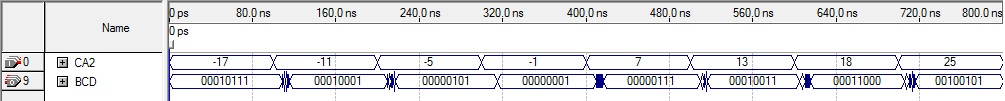
\includegraphics[scale=0.55]{../\projectname/assets/vwf/CA2_BCD_8B.jpg}
  \end{center}
  \caption{\label{fig:sim-\projectname-CA2_BCD_8B} Simulació per al bloc \textsf{CA2\_BCD\_8B}}
\end{contendfig}

La simulació del bloc es pot veure a la figura~\ref{fig:sim-\projectname-CA2_BCD_8B} (pàgina~\pageref{fig:sim-\projectname-CA2_BCD_8B}).

% FIXME

\vspace{1cm}
